\chapter{Algorithmic Approaches}

In this section, several algorithmic approaches to solving the Polyomino Assembly Problem with and without fixed seed tiles are investigated. First, we discuss the hardness of the investigated problems; subsequently, several algorithms are developed. The main focus is on heuristic search-based algorithms, specifically best-first search with various heuristics. Some of the developed heuristics are admissible, meaning that they never overestimate the distance to the target configuration and thus lead to an A* search, which finds sequences of optimal length as solutions, whereas other approaches give up on optimality in exchange for an improved runtime. Furthermore, during the expansion of the search tree, branches that provably cannot lead to a solution can be pruned in order to avoid unnecessary computations. This means, that the configuration represented by these nodes is never used for later expansion steps. Multiple pruning methods are investigated. In addition to the search-based algorithms, we propose an approach using RRTs. Finally, a method for shortening an existing solution is briefly examined.


\section{Hardness of the Problems}
The PSPACE-completeness of the Polyomino Assembly Problem without fixed seed tile follows directly from the PSPACE-completeness of the occupancy problem. For the Fixed Seed Tile Polyomino Assembly Problem, we show, that it is PSPACE-complete even under the conditions, that there are exactly as many tiles on the board as needed to assemble the target shape and the number of glues is constant.

\begin{theorem}
The Fixed Seed Tile Polyomino Assembly Problem is in PSPACE
\end{theorem}

\begin{proof}
Repeated, non-deterministic selection of control inputs until the target shape is assembled solves the problem and only requires us to store the current configuration. Therefore, the problem is in NPSPACE, which is equal to PSPACE.
\end{proof}

\begin{theorem}
The Fixed Seed Tile Polyomino Assembly Problem is PSPACE-hard
\end{theorem}

\begin{figure}
\centering
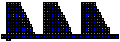
\includegraphics[width=\textwidth]{figures/hardnessproof.pdf}
\caption[Reduction of the $k$-region relocation problem to Fixed Seed Tile Polyomino Assembly Problem]{Reduction of the $k$-region relocation problem to the Fixed Seed Tile Polyomino Assembly Problem. The red square is the fixed seed tile, the yellow tile $t_{\text{reloc}}$ needs to be relocated $3$ positions to the right in order to assemble the target shape. The blue squares are other tiles. Figure recreated and adapted from \cite{Caballero2020a}.}
\label{fig:hardnessproof}
\end{figure}

\begin{proof}
To show PSPACE-hardness we adapt a proof from ~\cite{Caballero2020a} and reduce from the \emph{$k$-region relocation problem} of the full-tilt model~\cite{BalanzaMartinez2020}. In this problem, $k$ disjoint regions each contain a single tile. The goal is to move all $k$ tiles to the $1 \times 3$ region at the bottom of their respective component using tilt transformations. Analogous to \cite{Caballero2020a}, we start the reduction by connecting the $1 \times 3$ regions to a single bottom row and invert tile placement by placing tiles on all open spaces that did not contain a tile in the original instance of the $k$-region relocation problem. Additionally, we place a fixed seed tile $k$ positions to the right and $1$ down from the leftmost tile in the bottom row $t_{\text{reloc}}$, as shown in Figure \ref{fig:hardnessproof}. We assign glues as follows: The fixed seed tile has glue $A$ on all four edges. $t_{\text{reloc}}$ has glue $B$ on all edges. Every other tile has glue $C$ on all edges. Furthermore, we define the glue function $G$, such that $G(A,B) = G(B,C) = G(C,C) = 1$ and $G(X, Y) = 0$ for all other pairs of glues $X, Y$. Finally, we define the target shape as all open spaces inside the connected region, except for the $k$ leftmost positions in the bottom row. Now a solution to the constructed instance of the Fixed Seed Tile Polyomino Assembly Problem corresponds to a solution to the original instance of the $k$-region relocation problem. The key idea is, that tiles can only bond if they are connected to the seed tile and that only $t_{\text{reloc}}$ can directly bond with the seed tile according to the glue function. Therefore, $t_{\text{reloc}}$ must be relocated $k$ positions to the right, which was shown to solve the original $k$-region relocation problem (in \cite{Caballero2020a}). Conversely, once $t_{\text{reloc}}$ has been successfully moved $k$ spaces to the right, the target shape is immediately assembled, as all open spaces, except the $k$ leftmost positions in the bottom row, are filled with tiles that can bond according to the glue function and are connected to the fixed seed tile via $t_{\text{reloc}}$.
\end{proof}

\begin{corollary}
The Fixed Seed Tile Polyomino Assembly Problem with extra tiles is PSPACE-hard.
\end{corollary}

Note that this leaves open whether the problem is PSPACE-hard when only a single glue other than the \texttt{null} glue is allowed.

\section {Best-First Search}
We explore two different approaches to best-first search. The first approach aims to build the target polyomino directly by minimizing a function of the distances of tiles to the target shape. The second approach aims to build the target polyomino iteratively by adding one tile after the other, while at the same time attempting to keep the remaining tiles separate. \par
To avoid repeatedly visiting the same configuration, information that allows the identification of previously visited board positions must be stored. In our implementation, we compute and store hash values based on the positions and glues of all tiles in order to uniquely identify configurations on a given board.

\subsection {All Tiles at the Same Time}
As the basis for the following heuristic functions, the concept of the $n$ nearest available tiles is used. \par
Given an instance of the Polyomino Assembly Problem with configuration $C = (B, T)$ and a target shape $X$ with $|X| = n$. Let $T_{\text{available}}$ be the set of tiles which are part of a polyomino $P$ for which a path exists that avoids blocked positions in $B$ and along which $P$ can be moved to a position where it is contained in $X$. Assuming that $|X| \leq |T_{\text{available}}|$, $d$ is the distance of the $n$-th nearest tile to the target shape in $T_{\text{available}}$ and $T^\prime= \{t \in T_{ \text{available}} \mid d(t) \leq d \}$.
The branch can be pruned, if $|T_{\text{available}}|$ contains fewer tiles than needed for the target shape

\paragraph{Greatest Distance Heuristic:}
The Greatest Distance heuristic (GD) is an admissible heuristic that can be used in combination with the A* search algorithm. In the resulting algorithm, the value of the heuristic is added to the distance of the current configuration from the initial configuration, i.e., the number of moves required to get to the current configuration. \par
Given a configuration $C$ and a target shape $X$ the heuristic function $h_{\text{GD}}$ is defined as
\begin{equation}
h_{\text{GD}}(C, X) \coloneqq \max_{t \in T^\prime}{d(t)}.
\end{equation}
It is apparent that the greatest distance among the $n$ nearest tiles is a valid lower bound for the number of required moves because every move can reduce the distance of each tile to the target shape by a maximum of $1$ and at least $n$ tiles must reach the target shape in order to complete the assembly. Furthermore, tiles that cannot be part of the target polyomino because they are part of a polyomino that does not fit into the target shape or does not have an unblocked path to the target shape can be ignored. In order to decide if a given tile is in $T_{\text{available}}$, our implementation remembers for each polyomino if it is able to reach the target shape and fits into the target shape. These functions are only reevaluated whenever the polyomino changes. Since polyominoes are expected to change relatively infrequently, the computational overhead should be limited. \par
A heuristic is called consistent if the estimated distance of a node to the goal is never greater than the estimate for any neighboring node plus the cost of reaching that neighbor. As a consequence, an A* search using a consistent heuristic will find the shortest path to any node when that node is processed for the first time. Since a single step, which has a cost of $1$, applied to a configuration reduces the heuristic value of GD by a maximum of $1$ GD is consistent.
\paragraph{Average Distance Heuristic:}
Similar to GD the Average Distance heuristic (AD) is computed based on the distance of the $n$ nearest tiles that can potentially be part of the target shape. A disadvantage of GD is that it only takes into account the greatest distance among the $n$ nearest available tiles and disregards the distances of the closer tiles, which can cause GD to overestimate moves that bring the most distant tile closer but increase the distance of many other tiles to the target shape. The Average Distance heuristic attempts to also take into account the distance of the closer tiles by using the arithmetic mean.
\begin{equation}
h_{\text{AD}}(C, X) \coloneqq \dfrac {\sum_{t \in T^\prime}{d(t)}} {|T^\prime|}
\end{equation}
Following the same logic as above, $h_{\text{AD}}$ is also a consistent heuristic.

\paragraph{Gready Greatest Distance and Greedy Average Distance Heuristic:}
Both $h_{\text{GD}}$ and $h_{\text{AD}}$ can be used in combination with a greedy best-first search approach by not adding the distance from the initial configuration to the heuristic value. If the heuristics are used in this context, we refer to the resulting algorithms as Gready Greatest Distance (GGD) and Greedy Average Distance (GAD) respectively. The idea of this approach is to give up the optimality of the solution in order to potentially improve the execution speed.

\paragraph{Weighted Sum of Distances Heuristic:}
The Weighted Sum of Distances heuristic (WSD) is a non-admissible heuristic, that is an attempt at a generalization of GGD and GAD. While GGD only takes into account the distance of the most distant tile, in GAD the distances of all $n$ nearest available tiles each have the same impact on the heuristic value. WSD allows adjusting the influence that a tile has on the heuristic value based on its distance to the target shape by introducing an exponent $e \in \left[1,\infty\right)$.
\begin{equation}
h_{\text{WSD}} \coloneqq \sum_{t \in T^\prime}{d(t)^e}
\end{equation}
For $e = 1$ WSD behaves equivalently to GAD, whereas for greater $e$, tiles with a greater distance to the target shape have an increased impact on the heuristic function. For a sufficiently large $e$, the heuristic value is essentially defined by the greatest distance among tiles and WSD behaves similar to GGD.

\paragraph{Pruning methods:}
There are multiple pruning methods that can be used together with the all-tiles-at-the-same-time approach. Firstly, if $|T_{\text{available}}| < n$, the configuration can never lead to a solution.
Furthermore, when it can be shown that there is no subset of existing polyominoes which can exactly cover the target shape, the branch can be pruned.
% In general, however, it is NP-complete to decide whether such a tiling of the target shape exists \cite{} and therefore it is not feasible to compute every time a polyomino changes.
Generally, however, it may not be computationally feasible to decide whether such a tiling of the target shape exists every time a polyomino changes.
In the case where there are exactly as many tiles on the board as needed to form the target shape, we determine if the $k$ largest polyominoes can be packed into the target shape. If this is not possible then the branch can be pruned. In our implementation $k = 3$ is selected.


\paragraph{Alternative Stop Condition:}
When the configuration contains exactly as many tiles as needed for the target polyomino, an alternative stop condition can be utilized, which sometimes gets to a solution after fewer expanded nodes.
If at any point during the heuristic search a configuration $C$ contains a single polyomino $P$ that fits exactly into the target shape and for which a path to the target shapes location exists, the sequence leading to $C$, concatenated with a shortest sequence that moves $P$ from its current location to the location of the target shape is a solution to the problem. The later sequence can be found through a breadth-first search. \par
A solution found in this way is not necessarily of optimal length, even if one of the A* search approaches with a consistent heuristic is used. However, it can only be longer than the optimal solution by at most $d_{max}$ steps, where $d_{max}$ is the greatest distance between any two open positions in $B$.


\subsection{One Tile at a Time}

In contrast to the all-tiles-at-the-same-time approach, the one-tile-at-a-time approach uses multiple consecutive best-first searches in order to add tiles one after another to a polyomino. For that reason, the heuristic function used for each of the separate best-first searches depends on the positions of the subassembly and the single tile that it is trying to combine. For that purpose, an implementation of the one-tile-at-a-time approach first needs to compute a set of tiles that can form the target shape and a building order in which these tiles can be added one at a time to construct the target polyomino. Each best-first search attempts to keep all tiles that are not involved in the current construction step separated from each other by pruning configurations with unwanted subassemblies. Importantly, this approach is not a complete solution to the (Fixed Seed Tile) Polyomino Assembly Problem, since it is not always possible to avoid creating multiple subassemblies even if the initial configuration only consists of trivial polyominoes (see Figure \ref{fig:subassemblies}). Furthermore, a found solution is unlikely to be optimal, even if each construction step consists of an A* search with a consistent heuristic. Nevertheless, this method can be effective in many cases. \par
All the following heuristics are used in combination with an A* search.

\begin{figure}
\centering
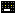
\includegraphics[width=0.5\textwidth]{figures/subassemblies.pdf}
\caption[Example of necessary subassemblies]{Example instance that requires multiple subassemblies to assemble the target shape (red-striped area) and thus cannot be solved using the one-tile-at-a-time approach.}
\label{fig:subassemblies}
\end{figure}

\paragraph{Minimum Moves to Polyomino heuristic:}
Given a configuration $C = (B, T)$, a target shape $X$ and a Polyomino $P$, the Minimum Moves to Polyomino (MMP) heuristic provides a lower bound on the number of moves required to move a selected tile $t= (p_t, g_t)$ to a position defined relative to the position of $P$. Let $x$ be the absolute coordinates of the target position in the current configuration. For the purpose of the best-first search, the selected target position is always adjacent to a tile in P. Assuming that the absolute target position does not overlap with an obstacle, the heuristic function is defined as follows:
\begin{equation}
h_{\text{MMP}}(C, X, t, x) \coloneqq \left\lceil \dfrac {d(t, x) - d_{1}(t, x)}{2} \right\rceil+ d_{1} (t, x)
\end{equation}
$h_{\text{MMP}}$ is a lower bound on the number of moves required to move $t$ to the target position relative to $P$.

\begin{proof}
A single step reduces the length of a shortest path from $t$ to the target position by a maximum of $2$ because both $t$ and $P$ each move at most one unit distance. However, a move that reduces the distance by $2$ can never reduce the taxicab distance between $t$ and the target position because both $t$ and $P$ must move during the step in order for the distance to be reduced by $2$. By the definition of the step transformation, both $t$ and $P$ must move $1$ unit in the same direction. Therefore, the taxicab distance remains unchanged.
Furthermore, this implies that a single step can reduce the taxicab distance by a maximum of $1$. In this case, one of the components must be stationary and therefore the length of a shortest path is reduced by at most $1$ too. Therefore, a solution needs to contain at least $d_{1} (t, x)$ moves that reduce the length of a shortest path by $1$. This leaves a distance of at least $d(t, x) - d_{1} (t, x)$, which can be reduced by a maximum of $2$ per step.
\end{proof}


\begin{figure}
\centering

\includegraphics[width=0.4\textwidth]{figures/distance.pdf}
\caption[Example for MMP distance]{An example for the MMP distance calculation. The length of the shortest path between the bottom tile and the target position is $9$. The taxicab distance is $3$. Therefore, at least $(9 - 3) \mathbin{/} 2 + 3 = 6$ steps are needed to combine the tiles in the intended way.}
\label{fig:distance}
\end{figure}

Note that the target position can overlap with an obstacle that the target polyomino is adjacent to. In this case, the length of the shortest path to $x$ is replaced by the length of the shortest path to an adjacent position minus $1$. \par
A disadvantage of this heuristic is that it requires knowledge about the pairwise distance of all open positions on the board. In our implementation, these distances are computed in the beginning through breadth-first searches starting on each open position. This is only feasible for small boards as the calculation is $O(m^3)$ where $m$ is the number of open positions, and the memory is $O(m^2)$.

\paragraph{Minimum Moves to Polyomino and Target heuristic:}
The Minimum Moves to Polyomino and Target heuristic (MMPT) tries to mitigate the requirement to compute pairwise distances. For that purpose, the number of required moves as estimated by MMP is only used for the calculation of the heuristic value if both the current subassembly and the selected tile are within some threshold distance $d_t$ of the target area. We define the target area $A$, as the set of all open positions that the finished target polyomino can cover with any of its tiles after a sequence of steps. The target area can be computed with a breadth-first search. The distance of a position $p$ to the target area is called $d_{\text{A}}(p)$ and defined as the length of a shortest path from $p$ (or the nearest open position that $p$ is adjacent to), to the nearest position in the target area.
If the current target position or the selected tile is not near the target area, the maximum distance of the two components to the target area is used as a basis for the heuristic value instead. In this case, to prioritize configurations where both components are near the target area, we apply a factor $w = |A|$. $w$ is proportional to the size of the target area to account for the greater possible distances within a larger target area.
Alternatively $w$ could be selected as the greatest distance within the target area.
\begin{equation}
h_{\text{MMPT}}(C, X, t, x) \coloneqq
\begin{cases}
h_{\text{MMP}}(C, X, t, x), & \text{if } d_{\text{A}}(p_t) \leq d_t \text{ and } d_{\text{A}}(x) \leq d_t\\
w \cdot \max(d_{\text{A}}(p_t), d_{\text{A}}(x)), & \text{otherwise}
\end{cases}
\end{equation}

This approach has two main advantages over MMP. Firstly, it only requires the computation of pairwise distances within the proximity of the target area. Secondly, MMP does not consider in what position the subassembly is formed in relation to the final position of the target shape. This can lead to the formation of subassemblies in locations from where they cannot reach the target shape anymore. In the MMP approach, such branches get pruned; however, the heuristic function does not actively avoid the creation of subassemblies outside the target area. In contrast, MMPT prioritizes forming subassemblies within the reachable area of the target shape.\par
Note that MMPT is not a consistent heuristic.


\paragraph{Distance to Fixed Position heuristic:}
In the case of a fixed seed tile, a much simpler heuristic can be used as a lower bound on the number of required moves to combine a selected tile with the fixed target polyomino.
Because the target position of the tile is fixed, each move can reduce the length of a shortest path from the tile to the target position by a maximum of $1$.
\begin{equation}
h_{\text{DFP}}(C, X, t, x) \coloneqq d(t, x)
\end{equation}
Additionally, during the computation of the shortest paths to the target position, the positions of tiles contained in the fixed polyomino, as well as neighboring positions that are impassable for the selected tile because of glues on the edges of a fixed tile can be marked as blocked.

\paragraph{Pruning methods:}
All of the one-tile-at-a-time approaches require the same two pruning methods. Firstly, a branch is pruned if its configuration contains an unwanted subassembly. Secondly, a branch is pruned if the correct subassembly is present, but is in a location from where it cannot reach a position where it is contained in the target shape.

\paragraph{Computation of the Building Order:}
To compute an order in which tiles can be added to the polyomino, a tiling of the target shape such that all tiles bond is determined using a brute-force algorithm.
Then a recursive backtracking algorithm that removes tiles from the polyomino one after the other is utilized. If all tiles can be removed from the polyomino in this way the reversed deconstruction order is a \emph{potential} building order. To determine if a tile can be removed two conditions are checked.
\begin{enumerate}
\item Do the remaining tiles form a polyomino that is connected by glues?
\item Does a path exist, along which the selected tile can be moved outside of the rectangular region minimally enclosing the polyomino, without being blocked by other tiles or the glues on their edges? This is determined through a breadth-first search.
\end{enumerate}
This approach is directly inspired by research on the constructibility of polyominoes under tilt transformations \cite{Becker2017}.
If this algorithm does not find a potential building order, it is attempted again with a different tiling of the polyomino until a potential building order is found or all possible tilings have been attempted.
A building order found in this way is not guaranteed to be realizable on the board of the problem instance. If any of the best-first searches during the motion planning process terminate without finding a solution, the solver is restarted with another building order.


\section{RRT}
The basic idea of an RRT search is to select a random configuration from the configuration space and expand the configuration in the current tree that is closest according to some cost-to-go function towards the selected configuration. When designing an RRT-based motion planning algorithm for the Polyomino Assembly Problem, the main challenge is to find a cost-to-go function that is fast to compute and provides a reasonable estimate of the distance between two configurations. \par
Let $C_1 = (B, T_1)$ and $C_2 = (B, T_2)$ be two configurations on the same board. 
As a first approach, we constructed a bipartite graph $G = (U, V, E)$ in which the vertices in $U$ represent the tiles from $T_1$ and the vertices in $V$ the tiles from $T_2$. A vertex in $U$ is connected to each vertex in $V$ that represents a tile with the same glues. The weight of the edge is the distance between the positions of the tiles.

Now the cost-to-go from $C_1$ to $C_2$ is estimated by the weight of the longest edge in a bottleneck matching. A bottleneck matching is a perfect matching that minimizes the length of the longest edge between $U$ and $V$. This is a lower bound on the number of steps needed to transform $C_1$ into $C_2$ because every tile in $C_1$ must be moved to a unique target position that contains a tile with the same glues in $C_2$ and each move can reduce the distance of each tile to its target position by a maximum of $1$.
However, the cost-to-go function needs to be evaluated many times during each expansion step of the RRT, and computing a bottleneck matching may be too expensive. Therefore a cost-to-go function that is quicker to compute was investigated. \par

For two tiles $t_1 = (p_1, g_1) \in T_1$ and $t_2 = (p_2, g_2) \in T_2$ we define
\begin{equation}
d_H(t_1, t_2) \coloneqq
\begin{cases}
d(p_1, p_2) , & \text{if } g_1 = g_2 \\
\infty , & \text{otherwise}
\end{cases}
\end{equation}
Then we define the distance between a tile $t$ and a set of tiles $S$ as $D_H(t, S) \coloneqq \min_{s \in S} d_H(s, t)$.
Note that $D_H(t_1, T_2) < \infty$ for any $t_1 \in T_1$, and vice versa, because both sets of tiles have the same sets of glues. \par

Now the cost-to-go-function between $C_1 = (B, T_1)$ and $C_2 = (B, T_2)$ is defined \mbox{equivalently} to the Hausdorff distance \cite{hausdorff} between the two sets of tiles.
\begin{equation}
D_H(C_1, C_2) \coloneqq \max \{	\max_{t_{1} \in T_{1}} d(t_1, T_2) , \max_{t_{2} \in T_{2}} d(t_2, T_1) \}
\end{equation}

Furthermore, if a polyomino exists in $C_1$ that does not fit into any polyomino of $C_2$ we set the cost-to-go to $\infty$. \par
Since the number of times the cost-to-go function is evaluated in each expansion step grows with the number of nodes in the RRT, we try to further mitigate the computational cost of repeatedly evaluating the cost-to-go function by keeping a sparser tree. This is achieved through a more expensive expansion step, which expands the closest node by multiple steps in the direction of the randomly selected configuration. For that purpose, a greedy best-first search with a limited number of iterations is used to minimize the cost-to-go. \par

A downside of both discussed cost-to-go functions is that they require knowledge about the pairwise distances between positions of the board. A potential solution is to use the taxicab distance instead of the length of a shortest path as the underlying distance metric. However, this would further decrease the accuracy of the estimated distance. \par

To estimate the distance to the goal, i.e., any configuration containing the target shape, a different metric must be used because the order of tiles within the target shape and the position of possible left-over tiles are not known. Therefore we choose the greatest distance among the $n$ nearest available tiles, as defined by the GD approach, as an estimate for the distance to the goal. The RRT nodes are kept in a list ordered by the distance to the goal. We bias the RRT search to expand the closest viable node directly towards the goal in $5\%$ of the expansion steps. For these expansion steps, the GGD approach with a limited number of iterations is used. If the distance from the selected node to the goal cannot be reduced in this way, the node is marked as dead and the next expansion towards the goal will use the next closest node. \par


\section {Solution Shortening}
Given two configurations $C_1$ and $C_2$ in which the tiles have the same positions relative to each other. Using a breadth-first search we can efficiently determine whether a sequence of inputs exists that transforms $C_1$ into $C_2$ and that preserves the relative positions of tiles after every step.
This can be used as a way to shorten a solution found by a motion planner as follows.\par
Start at the first position of the original sequence and find the last configuration that contains the same relative positions of tiles as the current configuration. If a sequence of steps between the two configurations shorter than the original sequence can be found using the above method, replace this part of the solution with the shorter sequence. Continue this process for the rest of the sequence.

